\documentclass[12pt]{scrartcl}
% Commit: ed8a9629

% ~^~^~^~^~^~^~^~^~^~^~^~^~^~^~^~^~^~^~^~^~^~^~^~^~^~^~^~^~^~^~ %

% Nia's Defs
% By Nia Madeline Heermance

% This document is updated over time.
% Feel free to use my defs if you find them useful.


% ~^~^~^~^~^~^~^~^~^~^~^~^~^~^~^~^~^~^~^~^~^~^~^~^~^~^~^~^~^~^~ %



% ...*...



% .:*~*:._.:*~*:._.:*~*:._.:*~*:._.:*~*:._.:*~*:._.:*~*:._.:*~*:. %

  % PREAMBLE
  
  % Document Class:
  % \documentclass{article}
  
  % _,.-'~'-.,__,.-'~' %

  % Packages:
  % Mathematics
    \usepackage{amsmath} % Math.
    \usepackage{amssymb} % Math Symbols.
    \usepackage{mathrsfs} % Fancy Math Fonts.
    \usepackage{amsthm} % Theorems.

  % Coding
    \usepackage{listings} % Coding Formats

  % Utility
    \usepackage{graphicx} % Figures.
    \usepackage{caption} % Hiding figure numbers.
    \usepackage{float} % For placing figures.
    \usepackage{enumerate} % Enumerate Entries.
    \usepackage{mathtools} % Boxing Aligned Answers.
    \usepackage{xparse} % Multiple Optional Arguments.
  
  % LaTeX Looks
    \usepackage[utf8]{inputenc} % UTF-8 Encoding
    \usepackage{microtype} % Allows stretching of letters for more happy boxes
    \usepackage{needspace} % Allows forcing of blocks to finish on the next page.
    \usepackage{color} % Different color keywords.
    \usepackage[colorlinks=true, linkcolor=blue, urlcolor=blue]{hyperref} % Links

  % _,.-'~'-.,__,.-'~' %

  % Document Settings:
    \usepackage{geometry} % Wide Margins.
    \setlength{\columnsep}{3cm}  % Setting the margins.
    \renewcommand*{\arraystretch}{1.2} % More spread out Matrices

    % Black Square at End of Proofs:
      \renewcommand\qedsymbol{$\blacksquare$} % Black Square.

    % Spacing:
      % Paragraph Spacing
        \parskip=0.5cm

      % Matrix Spacing
        \setlength\arraycolsep{8pt}
      \def\arraystretch{1.4}

      \makeatletter
      \renewenvironment{bmatrix}
      {\left[\mkern3.5mu\env@matrix}
      {\endmatrix\mkern3.5mu\right]}

      \renewenvironment{vmatrix}
      {\left\lvert\mkern5mu\env@matrix}
      {\endmatrix\mkern5mu\right\rvert}
      \makeatother

  % _,.-'~'-.,__,.-'~' %

  % Formatting Shortcuts
    
    % In-Line Format
      \newcommand{\disp}[1]{\displaystyle{#1}}
  

% .:*~*:._.:*~*:._.:*~*:._.:*~*:._.:*~*:._.:*~*:._.:*~*:._.:*~*:. %



% ...*... 



% .:*~*:._.:*~*:._.:*~*:._.:*~*:._.:*~*:._.:*~*:._.:*~*:._.:*~*:. %

  % SYMBOL SHORTCUTS
  % Bold Letters:
    % Lowercase:
      \newcommand{\ab}{\mathbf{a}}
      \newcommand{\bb}{\mathbf{b}}
      \newcommand{\cb}{\mathbf{c}}
      \newcommand{\db}{\mathbf{d}}
      \newcommand{\eb}{\mathbf{e}}
      \newcommand{\fb}{\mathbf{f}}
      \newcommand{\gb}{\mathbf{g}}
      \newcommand{\hb}{\mathbf{h}}
      \newcommand{\ib}{\mathbf{i}}
      \newcommand{\jb}{\mathbf{j}}
      \newcommand{\kb}{\mathbf{k}}
      \newcommand{\lb}{\mathbf{l}}
      \newcommand{\mb}{\mathbf{m}}
      \newcommand{\nb}{\mathbf{n}}
      \newcommand{\ob}{\mathbf{o}}
      \newcommand{\pb}{\mathbf{p}}
      \newcommand{\qb}{\mathbf{q}}
      \newcommand{\rb}{\mathbf{r}}
      \def\sb{\mathbf{s}}
      \newcommand{\tb}{\mathbf{t}}
      \newcommand{\ub}{\mathbf{u}}
      \newcommand{\vb}{\mathbf{v}}
      \newcommand{\wb}{\mathbf{w}}
      \newcommand{\xb}{\mathbf{x}}
      \newcommand{\yb}{\mathbf{y}}
      \newcommand{\zb}{\mathbf{z}}

    % Uppercase:
      \newcommand{\Ab}{\mathbf{A}}
      \newcommand{\Bb}{\mathbf{B}}
      \newcommand{\Cb}{\mathbf{C}}
      \newcommand{\Db}{\mathbf{D}}
      \newcommand{\Eb}{\mathbf{E}}
      \newcommand{\Fb}{\mathbf{F}}
      \newcommand{\Gb}{\mathbf{G}}
      \newcommand{\Hb}{\mathbf{H}}
      \newcommand{\Ib}{\mathbf{I}}
      \newcommand{\Jb}{\mathbf{J}}
      \newcommand{\Kb}{\mathbf{K}}
      \newcommand{\Lb}{\mathbf{L}}
      \newcommand{\Mb}{\mathbf{M}}
      \newcommand{\Nb}{\mathbf{N}}
      \newcommand{\Ob}{\mathbf{O}}
      \newcommand{\Pb}{\mathbf{P}}
      \newcommand{\Qb}{\mathbf{Q}}
      \newcommand{\Rb}{\mathbf{R}}
      \newcommand{\Sb}{\mathbf{S}}
      \newcommand{\Tb}{\mathbf{T}}
      \newcommand{\Ub}{\mathbf{U}}
      \newcommand{\Vb}{\mathbf{V}}
      \newcommand{\Wb}{\mathbf{W}}
      \newcommand{\Xb}{\mathbf{X}}
      \newcommand{\Yb}{\mathbf{Y}}
      \newcommand{\Zb}{\mathbf{Z}}

  % _,.-'~'-.,__,.-'~' %

  % Fancy Script:
    % Uppercase:
      \newcommand{\As}{\mathscr{A}}
      \newcommand{\Bs}{\mathscr{B}}
      \newcommand{\Cs}{\mathscr{C}}
      \newcommand{\Ds}{\mathscr{D}}
      \newcommand{\Es}{\mathscr{E}}
      \newcommand{\Fs}{\mathscr{F}}
      \newcommand{\Gs}{\mathscr{G}}
      \newcommand{\Hs}{\mathscr{H}}
      \newcommand{\Is}{\mathscr{I}}
      \newcommand{\Js}{\mathscr{J}}
      \newcommand{\Ks}{\mathscr{K}}
      \newcommand{\Ls}{\mathscr{L}}
      \newcommand{\Ms}{\mathscr{M}}
      \newcommand{\Ns}{\mathscr{N}}
      \newcommand{\Os}{\mathscr{O}}
      \newcommand{\Ps}{\mathscr{P}}
      \newcommand{\Qs}{\mathscr{Q}}
      \newcommand{\Rs}{\mathscr{R}}
      \newcommand{\Ss}{\mathscr{S}}
      \newcommand{\Ts}{\mathscr{T}}
      \newcommand{\Us}{\mathscr{U}}
      \newcommand{\Vs}{\mathscr{V}}
      \newcommand{\Ws}{\mathscr{W}}
      \newcommand{\Xs}{\mathscr{X}}
      \newcommand{\Ys}{\mathscr{Y}}
      \newcommand{\Zs}{\mathscr{Z}}
      
   % Less Fancy Script:
    % Uppercase:
      \newcommand{\Ac}{\mathcal{A}}
      \newcommand{\Bc}{\mathcal{B}}
      \newcommand{\Cc}{\mathcal{C}}
      \newcommand{\Dc}{\mathcal{D}}
      \newcommand{\Ec}{\mathcal{E}}
      \newcommand{\Fc}{\mathcal{F}}
      \newcommand{\Gc}{\mathcal{G}}
      \newcommand{\Hc}{\mathcal{H}}
      \newcommand{\Ic}{\mathcal{I}}
      \newcommand{\Jc}{\mathcal{J}}
      \newcommand{\Kc}{\mathcal{K}}
      \newcommand{\Lc}{\mathcal{L}}
      \newcommand{\Mc}{\mathcal{M}}
      \newcommand{\Nc}{\mathcal{N}}
      \newcommand{\Oc}{\mathcal{O}}
      \newcommand{\Pc}{\mathcal{P}}
      \newcommand{\Qc}{\mathcal{Q}}
      \newcommand{\Rc}{\mathcal{R}}
      \newcommand{\Sc}{\mathcal{S}}
      \newcommand{\Tc}{\mathcal{T}}
      \newcommand{\Uc}{\mathcal{U}}
      \newcommand{\Vc}{\mathcal{V}}
      \newcommand{\Wc}{\mathcal{W}}
      \newcommand{\Xc}{\mathcal{X}}
      \newcommand{\Yc}{\mathcal{Y}}
      \newcommand{\Zc}{\mathcal{Z}}

  % _,.-'~'-.,__,.-'~' %

  % Starred Letters
    % Lowercase:
      \def\ast{{a^*}}
      \newcommand{\bst}{{b^*}}
      \newcommand{\cst}{{c^*}}
      \newcommand{\dst}{{d^*}}
      \newcommand{\est}{{e^*}}
      \newcommand{\fst}{{f^*}}
      \newcommand{\gst}{{g^*}}
      \newcommand{\hst}{{h^*}}
      \newcommand{\ist}{{i^*}}
      \newcommand{\jst}{{j^*}}
      \newcommand{\kst}{{k^*}}
      \newcommand{\lst}{{l^*}}
      \newcommand{\mst}{{m^*}}
      \newcommand{\nst}{{n^*}}
      \newcommand{\ost}{{o^*}}
      \newcommand{\pst}{{p^*}}
      \newcommand{\qst}{{q^*}}
      \newcommand{\rst}{{r^*}}
      \newcommand{\sst}{{s^*}}
      \newcommand{\tst}{{t^*}}
      \newcommand{\ust}{{u^*}}
      \newcommand{\vst}{{v^*}}
      \newcommand{\wst}{{w^*}}
      \newcommand{\xst}{{x^*}}
      \newcommand{\yst}{{y^*}}
      \newcommand{\zst}{{z^*}}

    % Uppercase:
      \newcommand{\Ast}{{A^*}}
      \newcommand{\Bst}{{B^*}}
      \newcommand{\Cst}{{C^*}}
      \newcommand{\Dst}{{D^*}}
      \newcommand{\Est}{{E^*}}
      \newcommand{\Fst}{{F^*}}
      \newcommand{\Gst}{{G^*}}
      \newcommand{\Hst}{{H^*}}
      \newcommand{\Ist}{{I^*}}
      \newcommand{\Jst}{{J^*}}
      \newcommand{\Kst}{{K^*}}
      \newcommand{\Lst}{{L^*}}
      \newcommand{\Mst}{{M^*}}
      \newcommand{\Nst}{{N^*}}
      \newcommand{\Ost}{{O^*}}
      \newcommand{\Pst}{{P^*}}
      \newcommand{\Qst}{{Q^*}}
      \newcommand{\Rst}{{R^*}}
      \newcommand{\Sst}{{S^*}}
      \newcommand{\Tst}{{T^*}}
      \newcommand{\Ust}{{U^*}}
      \newcommand{\Vst}{{V^*}}
      \newcommand{\Wst}{{W^*}}
      \newcommand{\Xst}{{X^*}}
      \newcommand{\Yst}{{Y^*}}
      \newcommand{\Zst}{{Z^*}}

  % _,.-'~'-.,__,.-'~' %
  
  % Barred Letters
    % Lowercase:
      \newcommand{\abr}{\overline{a}}
      \newcommand{\bbr}{\overline{b}}
      \newcommand{\cbr}{\overline{c}}
      \newcommand{\dbr}{\overline{d}}
      \newcommand{\ebr}{\overline{e}}
      \newcommand{\fbr}{\overline{f}}
      \newcommand{\gbr}{\overline{g}}
      \newcommand{\hbr}{\overline{h}}
      \newcommand{\ibr}{\overline{i}}
      \newcommand{\jbr}{\overline{j}}
      \newcommand{\kbr}{\overline{k}}
      \newcommand{\lbr}{\overline{l}}
      \newcommand{\mbr}{\overline{m}}
      \newcommand{\nbr}{\overline{n}}
      \newcommand{\obr}{\overline{o}}
      \newcommand{\pbr}{\overline{p}}
      \newcommand{\qbr}{\overline{q}}
      \newcommand{\rbr}{\overline{r}}
      \newcommand{\sbr}{\overline{s}}
      \newcommand{\tbr}{\overline{t}}
      \newcommand{\ubr}{\overline{u}}
      \newcommand{\vbr}{\overline{v}}
      \newcommand{\wbr}{\overline{w}}
      \newcommand{\xbr}{\overline{x}}
      \newcommand{\ybr}{\overline{y}}
      \newcommand{\zbr}{\overline{z}}

    % Uppercase:
      \newcommand{\Abr}{\overline{A}}
      \newcommand{\Bbr}{\overline{B}}
      \newcommand{\Cbr}{\overline{C}}
      \newcommand{\Dbr}{\overline{D}}
      \newcommand{\Ebr}{\overline{E}}
      \newcommand{\Fbr}{\overline{F}}
      \newcommand{\Gbr}{\overline{G}}
      \newcommand{\Hbr}{\overline{H}}
      \newcommand{\Ibr}{\overline{I}}
      \newcommand{\Jbr}{\overline{J}}
      \newcommand{\Kbr}{\overline{K}}
      \newcommand{\Lbr}{\overline{L}}
      \newcommand{\Mbr}{\overline{M}}
      \newcommand{\Nbr}{\overline{N}}
      \newcommand{\Obr}{\overline{O}}
      \newcommand{\Pbr}{\overline{P}}
      \newcommand{\Qbr}{\overline{Q}}
      \newcommand{\Rbr}{\overline{R}}
      \newcommand{\Sbr}{\overline{S}}
      \newcommand{\Tbr}{\overline{T}}
      \newcommand{\Ubr}{\overline{U}}
      \newcommand{\Vbr}{\overline{V}}
      \newcommand{\Wbr}{\overline{W}}
      \newcommand{\Xbr}{\overline{X}}
      \newcommand{\Ybr}{\overline{Y}}
      \newcommand{\Zbr}{\overline{Z}}
      
% _,.-'~'-.,__,.-'~' %
  
  % Curved Letters
    % Lowercase:
      \newcommand{\afr}{\mathfrak{a}}
      \newcommand{\bfr}{\mathfrak{b}}
      \newcommand{\cfr}{\mathfrak{c}}
      \newcommand{\dfr}{\mathfrak{d}}
      \newcommand{\efr}{\mathfrak{e}}
      \newcommand{\ffr}{\mathfrak{f}}
      \newcommand{\gfr}{\mathfrak{g}}
      \newcommand{\hfr}{\mathfrak{h}}
      \newcommand{\ifr}{\mathfrak{i}}
      \newcommand{\jfr}{\mathfrak{j}}
      \newcommand{\kfr}{\mathfrak{k}}
      \newcommand{\lfr}{\mathfrak{l}}
      \newcommand{\mfr}{\mathfrak{m}}
      \newcommand{\nfr}{\mathfrak{n}}
      \newcommand{\ofr}{\mathfrak{o}}
      \newcommand{\pfr}{\mathfrak{p}}
      \newcommand{\qfr}{\mathfrak{q}}
      \newcommand{\rfr}{\mathfrak{r}}
      \newcommand{\sfr}{\mathfrak{s}}
      \newcommand{\tfr}{\mathfrak{t}}
      \newcommand{\ufr}{\mathfrak{u}}
      \newcommand{\vfr}{\mathfrak{v}}
      \newcommand{\wfr}{\mathfrak{w}}
      \newcommand{\xfr}{\mathfrak{x}}
      \newcommand{\yfr}{\mathfrak{y}}
      \newcommand{\zfr}{\mathfrak{z}}

    % Uppercase:
      \newcommand{\Afr}{\mathfrak{A}}
      \newcommand{\Bfr}{\mathfrak{B}}
      \newcommand{\Cfr}{\mathfrak{C}}
      \newcommand{\Dfr}{\mathfrak{D}}
      \newcommand{\Efr}{\mathfrak{E}}
      \newcommand{\Ffr}{\mathfrak{F}}
      \newcommand{\Gfr}{\mathfrak{G}}
      \newcommand{\Hfr}{\mathfrak{H}}
      \newcommand{\Ifr}{\mathfrak{I}}
      \newcommand{\Jfr}{\mathfrak{J}}
      \newcommand{\Kfr}{\mathfrak{K}}
      \newcommand{\Lfr}{\mathfrak{L}}
      \newcommand{\Mfr}{\mathfrak{M}}
      \newcommand{\Nfr}{\mathfrak{N}}
      \newcommand{\Ofr}{\mathfrak{O}}
      \newcommand{\Pfr}{\mathfrak{P}}
      \newcommand{\Qfr}{\mathfrak{Q}}
      \newcommand{\Rfr}{\mathfrak{R}}
      \newcommand{\Sfr}{\mathfrak{S}}
      \newcommand{\Tfr}{\mathfrak{T}}
      \newcommand{\Ufr}{\mathfrak{U}}
      \newcommand{\Vfr}{\mathfrak{V}}
      \newcommand{\Wfr}{\mathfrak{W}}
      \newcommand{\Xfr}{\mathfrak{X}}
      \newcommand{\Yfr}{\mathfrak{Y}}
      \newcommand{\Zfr}{\mathfrak{Z}}

  % _,.-'~'-.,__,.-'~' %
  
  % Greek Letters and Shortcuts:
    % Unbolded:
      % Lowercase:
        \newcommand{\al}{\alpha} % Alpha.
        \newcommand{\be}{\beta} % Beta.
        \newcommand{\gam}{\gamma} % Gamma.
        \newcommand{\del}{\delta} % Delta.
        \newcommand{\eps}{\varepsilon} % Epsilon.
        \newcommand{\zet}{\zeta} % Zeta.
        % \eta % Eta.
        \def\th{\theta} % Theta.
        \newcommand{\io}{\iota} % Iota.
        \newcommand{\kap}{\kappa} % Kappa.
        \newcommand{\lam}{\lambda} % Lambda.
        % \mu % Mu.
        % \nu % Nu.
        % \xi % Xi.
        % o % O.
        % \pi % Pi.
        % \rho % Rho.
        \newcommand{\sig}{\sigma} % Sigma.
        % \tau % Tau.
        \newcommand{\ups}{\upsilon} % Upsilon.
        \def\phi{\varphi} % Phi.
        % \chi % Chi.
        % \psi $ Psi.
        \newcommand{\om}{\omega} % Omega.

      % Uppercase:
        % A % Alpha.
        % B % Beta.
        \newcommand{\Gam}{\Gamma} % Gamma.
        \newcommand{\Del}{\Delta} % Delta.
        % E % Epsilon.
        \newcommand{\Zet}{\zeta} % Zeta.
        % \eta. % Eta.
        \newcommand{\Th}{\Theta} % Theta.
        % I % Iota.
        % K % Kappa.
        \newcommand{\Lam}{\Lambda} % Lambda.
        % M % Mu.
        % N % Nu.
        % \Xi % Xi.
        % O % O.
        % \Pi % Pi.
        % \rho % Rho.
        \newcommand{\Sig}{\Sigma} % Sigma.
        % T % Tau.
        \newcommand{\Ups}{\Upsilon} % Upsilon.
        \def\Phi{\Phi} % Phi.
        % X % Chi.
        % \Psi $ Psi.
        \newcommand{\Om}{\Omega} % Omega

    % Bolded:
       % Lowercase:
        \newcommand{\alb}{\boldsymbol{\al}} % Alpha.
        \newcommand{\beb}{\boldsymbol{\be}} % Beta.
        \newcommand{\gamb}{\boldsymbol{\gam}} % Gamma.
        \newcommand{\delb}{\boldsymbol{\del}} % Delta.
        \newcommand{\epsb}{\boldsymbol{\eps}} % Epsilon.
        \newcommand{\zetb}{\boldsymbol{\zet}} % Zeta.
        \newcommand{\etab}{\boldsymbol{\eta}} % Eta.
        \newcommand{\thb}{\boldsymbol{\th}} % Theta.
        \newcommand{\iob}{\boldsymbol{\io}} % Iota.
        \newcommand{\kapb}{\boldsymbol{\kap}} % Kappa.
        \newcommand{\lamb}{\boldsymbol{\lam}} % Lambda.
        \newcommand{\mub}{\boldsymbol{\mu}} % Mu.
        \newcommand{\nub}{\boldsymbol{\nu}} % Nu.
        \newcommand{\xib}{\boldsymbol{\xi}} % Xi.
        % \ob % O.
        \newcommand{\pib}{\boldsymbol{\pi}} % Pi.
        % \newcommand{\rhob}{\boldsymbol{\rho}} % Rho.
        \newcommand{\sigb}{\boldsymbol{\sig}} % Sigma.
        \newcommand{\taub}{\boldsymbol{\tau}} % Tau.
        \newcommand{\upsb}{\boldsymbol{\ups}} % Upsilon.
        \newcommand{\phib}{\boldsymbol{\phi}} % Phi.
        \newcommand{\chib}{\boldsymbol{\chi}} % Chi.
        \newcommand{\psib}{\boldsymbol{\psi}} % Psi.
        \newcommand{\omb}{\boldsymbol{\om}} % Omega.

      % Uppercase:
        % \Ab % Alpha.
        % \Bb % Beta.
        \newcommand{\Gamb}{\boldsymbol{\Gam}} % Gamma.
        \newcommand{\Delb}{\boldsymbol{\Del}} % Delta.
        % \Eb % Epsilon.
        \newcommand{\Zetb}{\boldsymbol{\Zet}} % Zeta.
        % \Hb % Eta.
        \newcommand{\Thb}{\boldsymbol{\Th}} % Theta.
        % \Ib % Iota.
        % \Kb % Kappa.
        \newcommand{\Lamb}{\boldsymbol{\Lam}} % Lambda.
        % \Mb % Mu.
        % \Nb % Nu.
        % \newcommand{\Xib}{\boldsymbol{\Xi}} % Xi.
        % \Ob % O.
        % \newcommand{\Pib}{\boldsymbol{\Pi}} % Pi.
        % \newcommand{\Rhob}{\boldsymbol{\Rho}} % Rho.
        \newcommand{\Sigb}{\boldsymbol{\Sig}} % Sigma.
        % \Tb % Tau.
        \newcommand{\Upsb}{\boldsymbol{\Ups}} % Upsilon.
        \newcommand{\Phib}{\boldsymbol{\Phi}} % Phi.
        % \Xb % Chi.
        % \newcommand{\Psib}{\boldsymbol{\Psi}} $ Psi.
        \newcommand{\Omb}{\boldsymbol{\Om}} % Omega.
        
    % Additional:
      \newcommand{\nab}{\nabla} % Nabla, inverted Delta.
      \newcommand{\nabb}{\boldsymbol{\nab}}


% .:*~*:._.:*~*:._.:*~*:._.:*~*:._.:*~*:._.:*~*:._.:*~*:._.:*~*:. %

  % BRACKETING

  % Left and Right:
    \def\l{\left}
    \def\r{\right}


  % Parentheses:
    % (
    \newcommand{\lp}{\left(} % Left (
    % )
    \newcommand{\rp}{\right)} % Right )


  % Square Brackets:
    % [
    \newcommand{\lbrc}{\left[} % Left [
    % ]
    \newcommand{\rbrc}{\right]} % Right ]


  % Braces:
    % \{
    \newcommand{\lbrs}{\left\{} % Left {
    % \}
    \newcommand{\rbrs}{\right\}} % Right }


  % Trianglar Bracket
    \newcommand{\la}{\langle} % Left Angle Bracket
    \newcommand{\ra}{\rangle} % Right Angle Bracket


  % Pipes:
    % | % Pipe
    \def\lv{\lvert} % Left Pipe
    \def\rv{\rvert} % Right Pipe


  % Magnitude
    % \| % Left Magnitude
    % \| % Right Magnitude



% .:*~*:._.:*~*:._.:*~*:._.:*~*:._.:*~*:._.:*~*:._.:*~*:._.:*~*:. %



% ...*...



% .:*~*:._.:*~*:._.:*~*:._.:*~*:._.:*~*:._.:*~*:._.:*~*:._.:*~*:. %

  % ARROWS
      
    % Arrow with Math
      \NewDocumentCommand{\xto}{o o} { 
        \IfValueTF{#1}{
          \IfValueTF{#2}{
            \xrightarrow[#2]{#1}
          }{
            \xrightarrow{#1}
          }
        }{
          \longrightarrow
        }
      }
    
    % Arrow with Text
      \NewDocumentCommand{\tto}{o o} { 
        \IfValueTF{#1}{
          \IfValueTF{#2}{
            \xrightarrow[\text{#2}]{\text{#1}}
          }{
            \xrightarrow{\text{#1}}
          }
        }{
          \to
        }
      }
    
    % Backwards Arrow
      \newcommand{\bto}{\,\leftarrow\,} 
      
     % Two Direction Arrow
      \newcommand{\lrto}{\leftrightarrow}




% .:*~*:._.:*~*:._.:*~*:._.:*~*:._.:*~*:._.:*~*:._.:*~*:._.:*~*:. %



% ...*...



% .:*~*:._.:*~*:._.:*~*:._.:*~*:._.:*~*:._.:*~*:._.:*~*:._.:*~*:. %

  % UTILITY
  
    % Quick words
      \newcommand{\andd}{\text{ and }}
      \newcommand{\forsm}{\text{ for some }}
      \newcommand{\orr}{\text{ or }}

    % Quick Formatting
      \newcommand{\textitbf}[1]{\textit{\textbf{#1}}}
      

% .:*~*:._.:*~*:._.:*~*:._.:*~*:._.:*~*:._.:*~*:._.:*~*:._.:*~*:. %



% ...*...



% .:*~*:._.:*~*:._.:*~*:._.:*~*:._.:*~*:._.:*~*:._.:*~*:._.:*~*:. %

  % SETS
  
    % Important Sets:
      \newcommand{\N}{\mathbb{N}} % Natural Numbers.
      \newcommand{\Z}{\mathbb{Z}} % Integers.
      \newcommand{\Q}{\mathbb{Q}} % Rational Numbers.
      \newcommand{\R}{\mathbb{R}} % Real Numbers.
      \newcommand{\C}{\mathbb{C}} % Complex Numbers.
      \newcommand{\empt}{\varnothing} % Empty Set.
    
    % Set Relations
      % Subset
        \newcommand{\subs}{\subset}
        \newcommand{\subeq}{\subseteq}
        \newcommand{\sups}{\supset}
        \newcommand{\supeq}{\supseteq}
      \newcommand{\nin}{\not\in}

    
    % Set Operations
      % Set Minus
      \newcommand{\setm}{\setminus}
      
      % Multiple Set Union
        \newcommand{\mun}{\bigcup}
        \newcommand{\munf}[1][k]{\mun_{#1 = 1}^\infty}
      % Multiple Set Intersection
        \newcommand{\mint}{\bigcap}
        \newcommand{\minf}[1][k]{\mun_{#1 = 1}^\infty}


% .:*~*:._.:*~*:._.:*~*:._.:*~*:._.:*~*:._.:*~*:._.:*~*:._.:*~*:. %



% ...*...



% .:*~*:._.:*~*:._.:*~*:._.:*~*:._.:*~*:._.:*~*:._.:*~*:._.:*~*:. %

  % THEOREMS

    % Lemma:
      \newtheorem{lemma}{Lemma}
      \newtheorem{theorem}{Theorem}

    % Definition
      \theoremstyle{definition} % Definition
      \newtheorem{definition}{Definition}


% .:*~*:._.:*~*:._.:*~*:._.:*~*:._.:*~*:._.:*~*:._.:*~*:._.:*~*:. %



% ...*...



% .:*~*:._.:*~*:._.:*~*:._.:*~*:._.:*~*:._.:*~*:._.:*~*:._.:*~*:. %

  % CALCULUS AND ANALYSIS

    % Set Tools
      \newcommand{\diam}{\text{diam}}
      
      % Interior
        \newcommand{\In}{\text{int }}
        
    % Function Tools
      \newcommand{\restr}[1]{|_{#1}}
      
    % Limits
      \newcommand{\limtinf}[1][n]{\lim_{#1\to\infty}}
      \newcommand{\limtz}[1][x]{\lim_{#1\to 0}}

    % Intergrals:
      % Differential D
      \newcommand{\dsl}{\:\textsl{d}}
      
      % \int % Single Integral
      \newcommand{\dint}{{\int \!\! \int \!\!}} % Double Integral.
      \newcommand{\tint}{{\int \!\! \int \!\! \int \!\!}} % Triple Integral.

      % Prebounded Integral
      \newcommand{\intb}{\int_a^b}

    % Derivatives:
      \newcommand{\parh}{\partial}
      \newcommand{\dv}[2]{\frac{d#1}{d#2}} % Single Derivative
      \newcommand{\dvop}[1][x]{\frac{d}{d#1}} % Single Derivative Operator
      \newcommand{\pdv}[2]{\frac{\partial #1}{\partial #2}} % Partial Derivative
      \newcommand{\pdvop}[1]{\frac{\partial}{\partial #1}} % Partial Derivative Operator
      
    % Special Operators
      \newcommand{\Jac}{\text{Jac}} % Jacobian
      \newcommand{\Curl}{\text{Curl}} % Curl

    % Convergence
      % Point-wise Convergence
        \newcommand{\pwto}{\tto[p.w.]}
      % Uniform Convergence
        \newcommand{\unif}{\tto[unif.]}
      
    % Measure
      % Outer Measure
        \newcommand{\omes}{{m_*}}
      

% .:*~*:._.:*~*:._.:*~*:._.:*~*:._.:*~*:._.:*~*:._.:*~*:._.:*~*:. %



% ...*...



% .:*~*:._.:*~*:._.:*~*:._.:*~*:._.:*~*:._.:*~*:._.:*~*:._.:*~*:. %

  % COMPLEX ANALYSIS
  
    % Components
      \newcommand{\re}{{\rm Re }~} % Real Component
      \newcommand{\im}{{\rm Im }~} % Imaginary Component

% .:*~*:._.:*~*:._.:*~*:._.:*~*:._.:*~*:._.:*~*:._.:*~*:._.:*~*:. %



% ...*...



% .:*~*:._.:*~*:._.:*~*:._.:*~*:._.:*~*:._.:*~*:._.:*~*:._.:*~*:. %

% LINEAR ALGEBRA

  % Bracketed Matrices:
    \NewDocumentCommand{\bmat}{o}{
      \IfValueTF{#1} {
        \begin{bmatrix}[#1]
      }{
        \begin{bmatrix}
      }
    }
    
    \newcommand{\emat}{\end{bmatrix}} % End Matrix
    
  % Determinant Matrices:
    \newcommand{\vbmat}{\begin{vmatrix}}
    \newcommand{\vemat}{\end{vmatrix}}
    
  % Augmented Matrices:
    \makeatletter
      \renewcommand*\env@matrix[1][*\c@MaxMatrixCols c]{%
	  \hskip -\arraycolsep
	  \let\@ifnextchar\new@ifnextchar
	   \array{#1}}
    \makeatother

    % And to display them:
      \def\Height{\vphantom{\begin{array}{c}a\cr a\cr a\cr\end{array}}} 
      \def\|{\!\!\smash{\left|\Height\right.}\!\!} 
      \def\Matrix#1{\left[\;\;\Height\begin{array}{rrrcr}#1\end{array}\;\;\right]}
    
  % Zero Vector
    \newcommand{\ozb}{\textbf{0}}
    
  % Operators
    \newcommand{\Span}{\text{span }}
    
    

% .:*~*:._.:*~*:._.:*~*:._.:*~*:._.:*~*:._.:*~*:._.:*~*:._.:*~*:. %



% ...*...



% .:*~*:._.:*~*:._.:*~*:._.:*~*:._.:*~*:._.:*~*:._.:*~*:._.:*~*:. %

% ABSTRACT ALGEBRA

  % Kernel
    \newcommand{\Ker}{\text{Ker}\:}


% .:*~*:._.:*~*:._.:*~*:._.:*~*:._.:*~*:._.:*~*:._.:*~*:._.:*~*:. %



% ...*...



% .:*~*:._.:*~*:._.:*~*:._.:*~*:._.:*~*:._.:*~*:._.:*~*:._.:*~*:. %

  % PROGRAMMING

    % Coding Fonts
      % Default teletype font does not support bold face
      \DeclareFixedFont{\telemed}{T1}{txtt}{m}{n}{12}  % Normal Text
      \DeclareFixedFont{\telebold}{T1}{txtt}{bx}{n}{12} % Bold Text
      
    % Coding Colors
    \definecolor{deepblue}{rgb}{0,0,0.5}
    \definecolor{deepred}{rgb}{0.6,0,0}
    \definecolor{deepgreen}{rgb}{0,0.5,0}

    % Generic Code
      \newcommand{\codel}[1]{\texttt{#1}} % In-Line Code

    % Python
      % Python Text styles
      \newcommand{\pystyleb}{
        \lstset{
          framesep=10pt,  % Increased from 5pt to 10pt
          language=Python,
          basicstyle=\telemed,
          morekeywords={self}, % Add more over time.
          keywordstyle=\telebold\color{deepblue},
          emph={}, % Custom highlighting
          emphstyle=\telebold\color{deepred},
          stringstyle=\color{deepgreen},
          frame=tb,
          showstringspaces=false
        }
      }
      \lstdefinestyle{pystylel}{
        language=Python,
        basicstyle=\ttfamily,
        keywordstyle=\color{deepblue},
        stringstyle=\color{deepgreen}
      }

      % Python Environment, allowing for optional styling like line numbers.
      \lstnewenvironment{python}[1][]
      {
        \vspace{\topsep}
        \needspace{2\baselineskip}
        \pystyleb
        \lstset{#1}
      }
      {
        \needspace{2\baselineskip}
        \vspace{\topsep}
      }

      \newcommand{\pythonl}[1]{\lstinline[style=pystylel]!#1!} % Python In-Line


% .:*~*:._.:*~*:._.:*~*:._.:*~*:._.:*~*:._.:*~*:._.:*~*:._.:*~*:.



% ...*...



% .:*~*:._.:*~*:._.:*~*:._.:*~*:._.:*~*:._.:*~*:._.:*~*:._.:*~*:. %

  % OTHER

    % Congruence:
      \newcommand{\teq}{\equiv} % Triple Equal Sign.
      \newcommand{\tneq}{\not\equiv} % Not Triple Equal Sign.
 
    % Inverse
      \newcommand{\inv}{{-1}} % -1 Grouped Together.


% .:*~*:._.:*~*:._.:*~*:._.:*~*:._.:*~*:._.:*~*:._.:*~*:._.:*~*:.


% ***
\parskip=0.5cm

\title{\vspace{-2em} Linear Equations Overview}
\author{}
\date{}

\begin{document}
\maketitle
\vspace{-6em}

\section*{What are linear equations?}
Linear Equations like the following
\[x + y + z = 1\]
have an $n$-dimensional plane as their graph:
\begin{figure}[H]
    \centering
    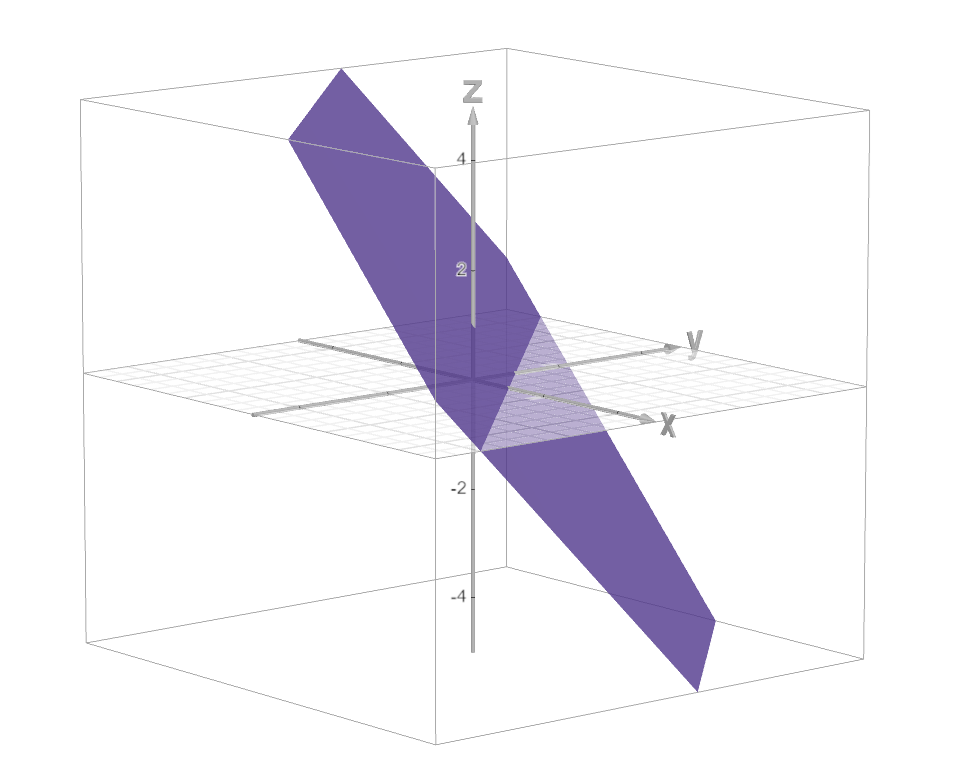
\includegraphics[scale=0.6]{x + y + z = 1.png}
    \caption*{$x + y + z = 1$}
\end{figure}
Because we have 3 variables, the graph is a $3-1=2$-dimensional plane, which is the typical plane we all know and love. We subtract 1 from the amount of dimensions because we can think of $z$ as a function of $x$ and $y,$ and that's 2 variables. So here, $z(x,y) = 1 - x - y.$ \footnote{Alternatively, we could think of $x$ as a function of $(y,z)$ or $y$ as a function of $(x,z).$} If the graph had 2 variables initially, it would be a $2-1=1$-dimensional plane, which is a line, and if it had 4 variables, it would be a $4-1=3$-dimensional plane, which would be a cube. And if it had 5 variables, it would be a 4-dimensional plane, which whould be a hyperplane!

Just like how a line extends forever, a 2D plane as visualized here extends out in all directions. We're only looking at a small piece of it. Linear equations create $n$-dimensional planes mathematically because the first derivatives with respect to each variable is constant. But intuitively, it's because if we set any of the variables to 0, say $x$, we would get the equation $y+z = 1$, which creates a line. If $x=1$, then we would have
\begin{align*}
    1 + y + z &= 1 \\
        y + z &= 0
\end{align*}
And if $x=2,$, we would have
\begin{align*}
    2 + y + z &= 1 \\
        y + z &= -1
\end{align*}
All of these equations are lines on the original plane $x+y+z=1$ we were looking at. So you can see that a 2-dimensional plane is just a bunch of 1-d planes, aka lines, all next to each other to make a rectangle. Similarly, we could think of a 3-dimensional planes as a bunch of 2D planes stacked on top of each other, like pieces of paper stacked to make a cube. This stacking effect is one of the main reasons we call these equations linear: there's no curvature, and we can simply stack the previous dimension to get the next plane.

\begin{figure}[H]
    \centering
    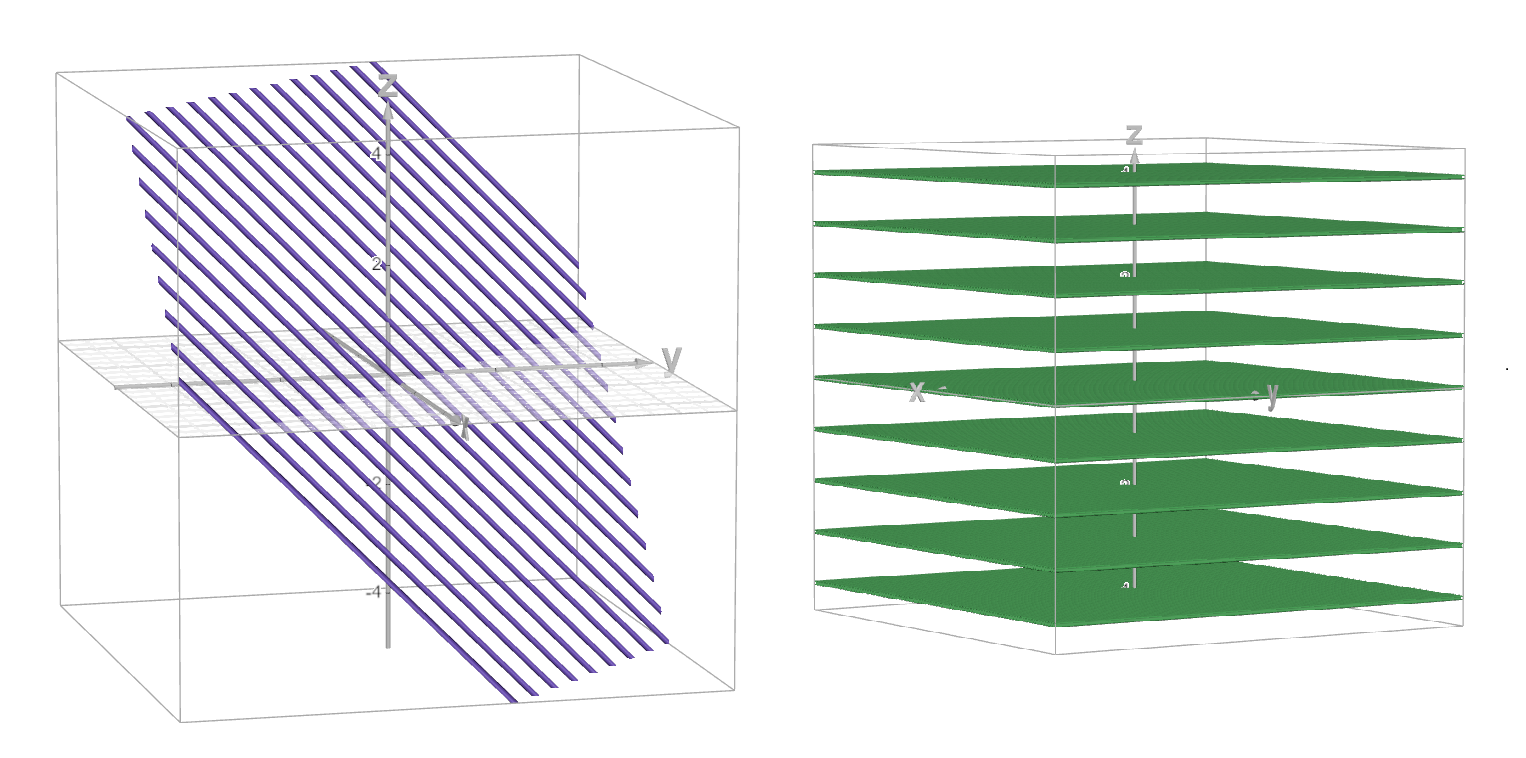
\includegraphics[scale=0.4]{Planes Make the Next Dimension.png}
    \caption*{Infinite lines make a plane. Infinite planes make a cube.}
\end{figure}

Okay, that explanation is good and all, but we were just looking at $x + y + z = 1,$ where each variables has a coefficient and the final number is 1. What happens if we change the final number?

Well, if $x,y=0$, then $x+y+z=1$ becomes $z=1$. Similarly, when $y,z=0,$ the equation becomes $x=1,$ and when $x,z=0$, the equation becomes $y=1.$ So the final number controls the axis intercepts.
\begin{figure}[H]
    \centering
    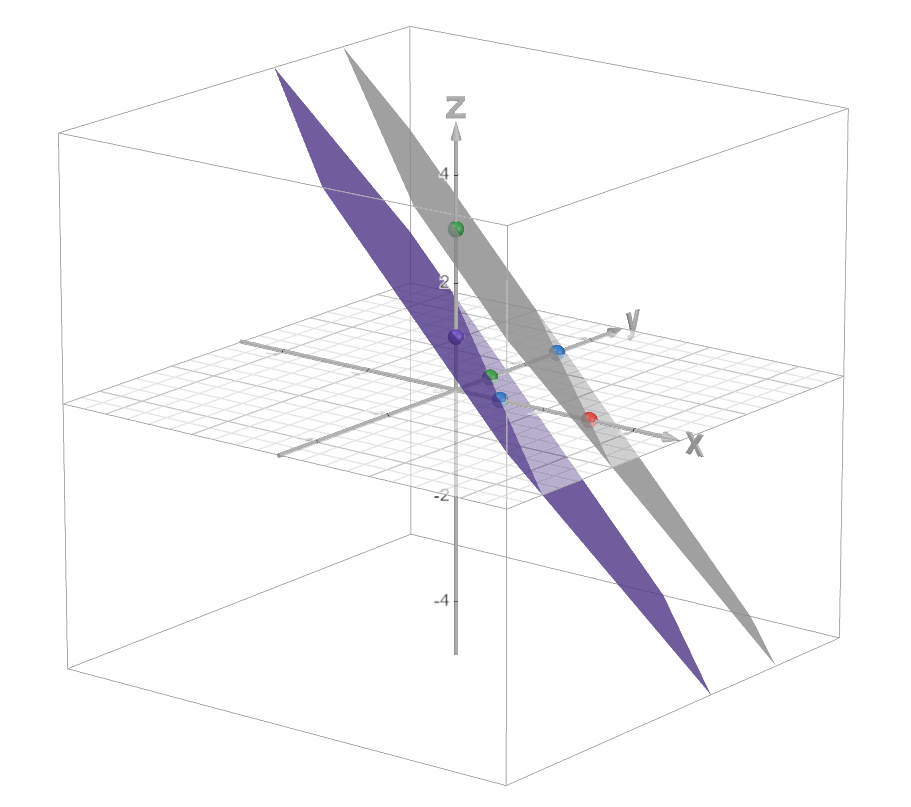
\includegraphics[scale=0.5]{Intercepts of Linear Equations.png}
    \caption*{$x+y+z=1\quad$ and $\quad x+y+z=3.$}
\end{figure}
Alright, so what do the coefficients do? Consider the equation $x+y+2z = 1.$ Because of the $2$ the slop is actually slower in the $z$ direction, as if we set $x=0$, we get $z = \frac{1}{2} - \frac{1}{2}y$, and if we set $y=0$, we get $z = \frac{1}{2} - \frac{1}{2}x.$ So the larger the coefficient, the smaller the relative slope in that axis direction.

\begin{figure}[H]
    \centering
    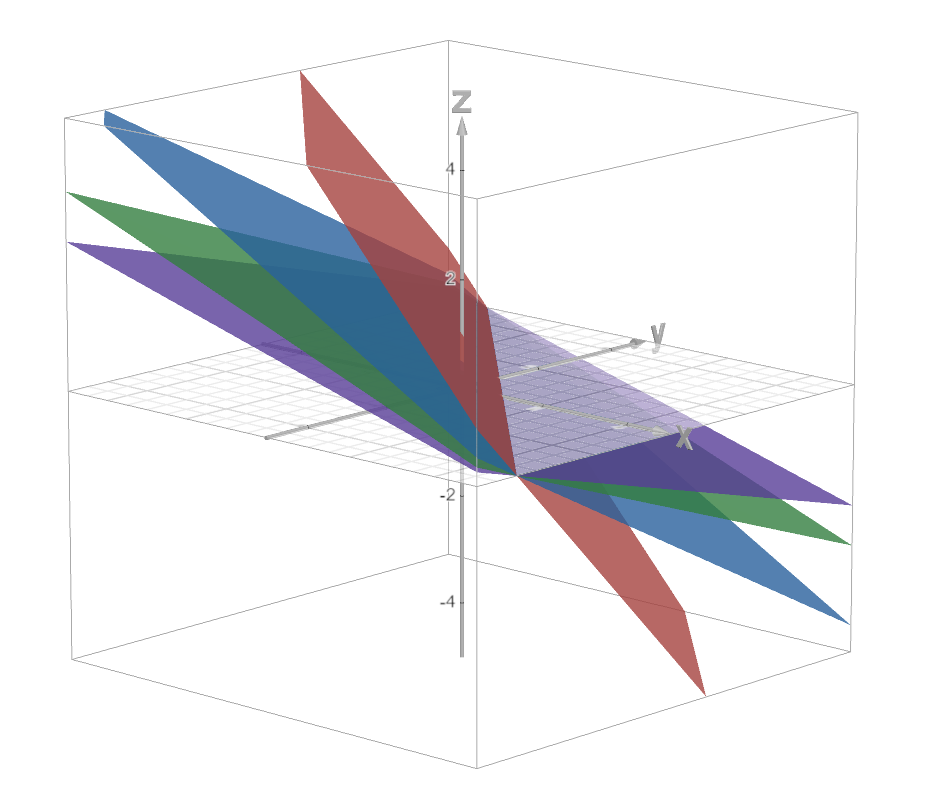
\includegraphics[scale=0.35]{Coefficient Affects Slope in that Axis.png}
    \caption*{Red is $x+y+z=1$, \: purple is $x+y+4z=1$.\quad Blue is $2z$, \: green is $3z$.}
\end{figure}

\subsubsection*{Overview}
\begin{itemize}
    \item Linear equations of $n$ variables represent $n-1$ dimensional planes.
    \item An $n$ dimensional plane is made out of infinite $n-1$ dimensional planes stacked on top of each other.
    \item The final constant determines the intercepts
    \item The coefficients on the variables determine the slope in that direciton, which overall controls the rotation of the plane
\end{itemize}

\newpage
\section*{Solving a System of Equations}
Consider the following equations:
\begin{align*}
    2x + y + z &= 2 \\
    x + 2y - z &= 3 \\
    -x - 3y + 4z &= 2
\end{align*}
We know that in algebra, it's valid to add equations together and to multiply both sides of an equation by a number. The order of how we listed the equations above doesn't suddenly change the planes, so the solution will stay the same if we list them in a different order by swapping two of them.

\vspace{-1em}
\begin{align*}
    x + 2y - z &= 3 \\
    2x + y + z &= 2 \\
    -x - 3y + 4z &= 2.
\end{align*}
\begin{center}
    The two equations are swapped...and the solution doesn't change.
\end{center}
\medskip

These three operations---multiplying by a number (also called a scalar), adding equations together, and swapping equations in the order we list them---are all valid algebraic procedures, so when we represent the system as a matrix, we are allowed to do these operations. We call them the \textit{elementary row operations}.

The matrix for the system above is:

\[\bmat[ccc|c] 2 & 1 & 1 & 2 \\ 1 & 2 & -1 & 3 \\ -1 & -3 & 4 & 2 \emat\]

You may be wondering why we don't add numbers or variables to both sides of an equation to help with solving. Our row operations only allow adding a whole other equation to our equation, not adding just numbers or variables to equation. However, we can of course do that! It's completely algebraically valid. It's just that, if we say, subtract 2 from equation 1,
\begin{align*}
    2x + y + z &= 2\\
    -2 \quad \: &\:\:-2 \\
    2x + y + z - 2 &= 0,
\end{align*}
well, we'll just have to add 2 again in order to get the equation in the form $ax + by + cz = d$ in order to get the top right entry in the matrix, which just means adding 2 all over again. Similarly, if we wanted to, say, solve for $z,$ we could subtract $2x$ and $y$ and get
\begin{align*}
    2x + y + z &= 2\\
    \text{$-$}2x \:\:\, \text{$-$}y\quad\:\: &\quad \: \text{$-$}2x \quad \text{$-$}y \\
   z &= 2 - 2x - y,
\end{align*}
This would be super useful if we were solving the equation with plain algebra! But because we want to solve an equation with a matrix, we would still have to convert the equation back to $ax + by + cz = d$ in order to get the entries for the first row of the matrix, undoing our progress.

So it turns out that with a matrix and the elementary row operations, we can solve a system of equations without having to add numbers or variables to an equation (instead, we add a whole entire other row equation). Adding numbers or variables to an equation is the main operation we do in normal algebra, so it may feel a bit weird that we don't need that operation in matrix form. However, once you're in row-echelon form, plain-old algebra is useful, but not before then.\footnotemark

\footnotetext{More precisely, we only add equations already in our system of equations to other equations in our system of equations. We don't add other equations to equations in our system of equations, as it wouldn't affect the entries in our matrix. When I said variables and numbers, these are equations too, just of the form $a=a$. Adding equations not in our system of equations is only useful once we're doing the small amount of algebra at the end of a row-echelon form solve.}

So now that we know the algebraic operations useful to us (which is adding equations to another equation, multiplying by a scalar, and swapping equations in our list), we're ready to simplify the matrix! Our goal is to get to the form:

\newpage
\[\begin{bmatrix}[ccc|c]
    1 & 0 & 0 & \text{some expression} \\
    0 & 1 & 0 & \text{another expression} \\
    0 & 0 & 1 & \text{a third expression}
\end{bmatrix}\]

This is because we would have $x + 0y + 0z =$ some expression, so $x =$ some expression. We would have the answer for $x$ that we could read right off the matrix! Similarly, $y =$ another expression and $z =$ a third expression. So let's begin row reducing.

When looking at the matrix, which I have repeated for convience,
\[\begin{bmatrix}[ccc|c]
    2 & 1 & 1 & 2 \\
    1 & 2 & -1 & 3 \\
    -1 & -3 & 4 & 2
\end{bmatrix}\]
you should think about which row has its first column closest to 1. In this case, it is row 2, as its column 1 entry already is 1. So if we swap rows 1 and 2, we have the top left done.
\[
    \begin{bmatrix}[ccc|c]
        2 & 1 & 1 & 2 \\
        1 & 2 & -1 & 3 \\
        -1 & -3 & 4 & 2
    \end{bmatrix}
    \xto[R_1 \lrto R_2]
    \begin{bmatrix}[ccc|c]
        1 & 2 & -1 & 3 \\
        2 & 1 & 1 & 2 \\
        -1 & -3 & 4 & 2
    \end{bmatrix}
\]
Next, we got to make it 0 in the first column for the new row 2 and also row 3:
\begin{align*}
    \begin{bmatrix}[ccc|c]
        1 & 2 & -1 & 3 \\
        2 & 1 & 1 & 2 \\
        -1 & -3 & 4 & 2
    \end{bmatrix}&\\
    \xto[R_2 \to R_2 - 2R_1][R_3 \to R_3 + R_1]&
    \begin{bmatrix}[ccc|c]
        1 & 2 & -1 & 3 \\
        0 & 1 - 2 \cdot 2 & 1 - 2 \cdot -1 & 2 - 2 \cdot 3 \\
        0 & -1 & 3 & 5
    \end{bmatrix} \\
    =\quad\:\:\: &
    \begin{bmatrix}[ccc|c]
        1 & 2 & -1 & 3 \\
        0 & -3 & 3 & -4 \\
        0 & -1 & 3 & 5
    \end{bmatrix}
\end{align*}

Now we look at rows 2 and 3 and decide which row is closest to 1 in the second column. We see that row 3 has $-1$ in its second column, which we can easily fix by multiplying by $-1.$ So we will swap rows 2 and 3 and then multiply the new row 2 by -1.
\footnote{Notice that we didn't consider swapping row 1 at all because we already have chosen row 1 to stay as the top row due to the 1 in column 1.}
\begin{align*}
    \begin{bmatrix}[ccc|c]
        1 & 2 & -1 & 3 \\
        0 & -3 & 3 & -4 \\
        0 & -1 & 3 & 5
    \end{bmatrix}
    \xto[R_2 \lrto R_3]&
    \begin{bmatrix}[ccc|c]
        1 & 2 & -1 & 3 \\
        0 & -1 & 3 & 5 \\
        0 & -3 & 3 & -4
    \end{bmatrix} \\
    \xto[R_2 \to \: -R_2]&
    \begin{bmatrix}[ccc|c]
        1 & 2 & -1 & 3 \\
        0 & 1 & -3 & -5 \\
        0 & -3 & 3 & -4
    \end{bmatrix}
\end{align*}
Now we need to get rid of the 2 in row 1 column 2 and the $-3$ in row 3 column 2. We'll get rid of the 2 later if we decide to go all the way to reduced row-echelon form. Recall that reduced row-echelon form and row-echelon form are ways of making the end algebra we have to do easier. With row-echelon form, we have to do a little easy algebra at the end, but with reduced row-echelon form, the solution is literally in the matrix so we don't need to do any algebra.

Continuing on,
\begin{align*}
    \begin{bmatrix}[ccc|c]
        1 & 2 & -1 & 3 \\
        0 & 1 & -3 & -5 \\
        0 & -3 & 3 & -4
    \end{bmatrix}&\\
    \xto[R_3 \to R_3 + 3R_2]&
    \begin{bmatrix}[ccc|c]
        1 & 2 & -1 & 3 \\
        0 & 1 & -3 & -5 \\
        0 & 0 & 3 + 3 \cdot -3 & -4 + 3 \cdot -5
    \end{bmatrix} \\
    =\quad\:\:\:&
    \begin{bmatrix}[ccc|c]
        1 & 2 & -1 & 3 \\
        0 & 1 & -3 & -5 \\
        0 & 0 & -6 & -19
    \end{bmatrix}
\end{align*}
We've delayed creating fractions as long as possible by swapping rows. But at this point, we're forced to divide row 3 by $-4$ in order to get a $z =$ expression:
\[
    \begin{bmatrix}[ccc|c]
        1 & 2 & -1 & 3 \\
        0 & 1 & -3 & -5 \\
        0 & 0 & -6 & -19
    \end{bmatrix}
    \xto[R_3 \to R_3/-4]
    \begin{bmatrix}[ccc|c]
        1 & 2 & -1 & 3 \\
        0 & 1 & -3 & -5 \\
        0 & 0 & 1 & 19/6
    \end{bmatrix}
\]
At this point, we have row-echelon form because we have 0s beneaths our main diagnonal. These 0s make the final algebra simple, \textbf{which we always do from bottom equation to top equation}:
\begin{align*}
    z &= 19/6. \\
    \\
    y - 3z &= -5 \\
    y &= -5 + 3\frac{19}{6}\\
    &= \frac{-30 + 30 + 27}{6}\\
    &= 27/6 = 9/2.
    \\
    x  + 2y - z &= 3 \\
    x &= 3 - 2\frac{27}{6} + \frac{19}{6} \\
    &= \frac{18 - 54 + 19}{6} \\
    &= -17/6.
\end{align*}
Notice how we never needed to go backwards and plug $x$ into the row 2 or row 3 equation, nor did we need to plug $y$ into the row 3 equation. This is why row-echelon form is so convient: the 0s mean we can just solve the equations bottom to top rather than having to jump back and forthe. Reduced row-echelon form would have allowed us to read the answers for $x,y,z$ right off the matrix, but this final algebra was easy enough so I stopped early as practice.

\newpage
\subsubsection*{Overview}
\begin{itemize}
    \item The ``elementary row operations'' are really just valid algebraic manipulations useful with matrices. We multiply equations by a number, add them to each other, and swap the equations order in our list.
    \item When row-reducing, switch rows so that the row with the closest entry to 1 is now on the main diagnoal.
    \item Avoid fractions for as long as possible to avoid arithmetic mistakes.
    \item Row-echelon form and reduced row-echelon form are just states a matrix can be that allows for simple algebra. Row-echelon form means the algebra allows you to go from bottom to top without jumping around, while reduced row-echelon form has the solution in the matrix itself.
\end{itemize}

\newpage
\section*{But what do solutions to linear equations mean geometrically?}
Consider this system:
\begin{align*}
    x + y + z &= 2 \\
    2x + y - z &= 3 \\
    -x + y + z &= 2
\end{align*}
We already know that 3 variable linear equations create 2D planes in 3D space. But what does the solution look like?

First, we'll solve this system. I won't go over the process in detail as the thinking you should have during the process was talked about in the previous seection and will be discussed further in a future section:
\begin{align*}
    \begin{bmatrix}[ccc|c]
       1 & 1 & 1 & 2 \\
       2 & 1 & -1 & 3 \\
       -1 & 1 & 1 & 2 
    \end{bmatrix}
    \xto[R_2 \to R_2 - 2R_1][R_3 \to R_3 + R_1]&
    \begin{bmatrix}[ccc|c]
        1 & 1 & 1 & 2 \\
        0 & -1 & -3 & -1 \\
        0 & 2 & 2 & 4
    \end{bmatrix} \\
    \xto[R_3 \to R_3 + 2R_2][R_2 \to -R_2]&
    \begin{bmatrix}[ccc|c]
        1 & 1 & 1 & 2 \\
        0 & 1 & 3 & 1 \\
        0 & 0 & -4 & 2
    \end{bmatrix}
\end{align*}
Then $-4z = 2$, so $z = -1/2.$ So $y = 1 + 3/2 = 5/2.$ Finally $x = 2 + 1/2 - 5/2 = 2 - 2 = 0$. Thus the solution is $(0, 5/2, -1/2),$ and we can see this solution is geometrically the intersection of the three planes:

\begin{figure}[H]
    \centering
    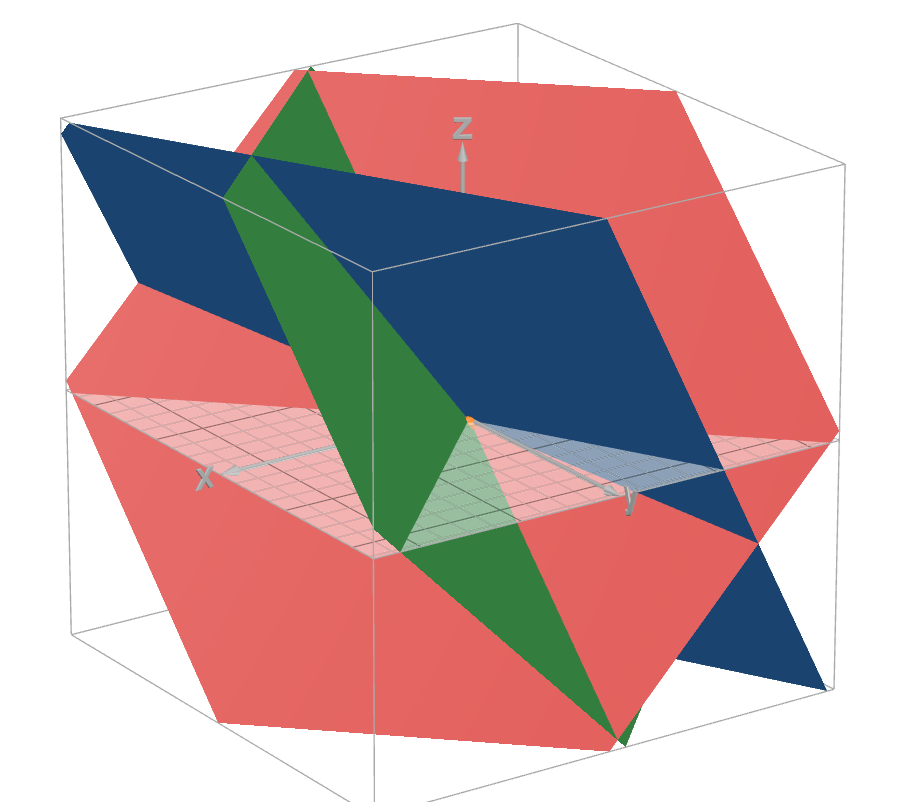
\includegraphics[scale=0.4]{Another Intercept of Three Planes.png}
    \caption*{Notice that the intercept, marked by the orange point, is slightly below the $xy$ plane thanks to the negative $z$. The point is at the y-axis thanks to $x=0$ and it's near the origin thanks to $y = 5/2$ being relatively small.}
\end{figure}

When all your plane intersect at a single point, we say the system has one solution. The question is how many planes do we need to have the intersection be one point? With two 2D planes, the intersection is a line, a 1D plane:
\begin{figure}[H]
    \centering
    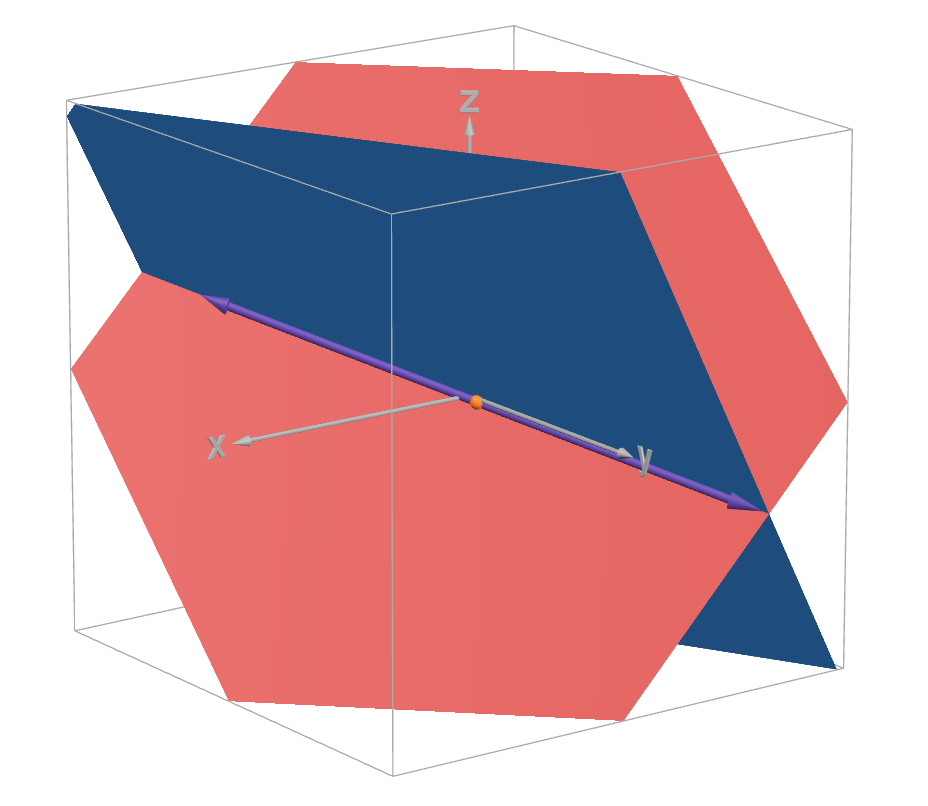
\includegraphics[scale=0.4]{Intercept of Two Planes.png}
    \caption*{Two 2D planes intersect along along a 1D plane.}
\end{figure}
But three 2D planes creates an intersection of a single point, a 0D plane. Just as you need $n$ equations to solve for $n$ variables, you need an $n$ amount of $n-1$ dimenstional planes to solve for a single point. Why $n-1$ and not $n$? 1 2D plane has the solution of the whole plane as the entire plane is of course always intersecting itself. 2 2D planes intersect at a 1D plane. And 3 2D planes intersect at a point. We went from a 2D solution to a 1D solution to a 0D (a point) solution. That's 3 scenarios, hence why we need 3 equations that associate with 3 planes to determine which scenario we're in, just like how we needed 3 equations to solve for 3 variables.

So two 2D planes intersect at a line. But I lied slightly. Consider the following system:
\begin{align*}
    3x + 2y - z &= 5, \\
    12x + 8y - 4z &= 20.
\end{align*}
The second equation is the first equation times 4. They have the same possible $(x,y,z)$ coordinates, so they represent the same plane! So 2 planes can intersect at a line or be the same plane.

Similarly, while 3 2D planes could intersect at a point, they could also

\begin{minipage}{0.48\textwidth}
    \begin{center}\raisebox{0pt}[1.95ex][0pt]{intersect at a line,}\end{center}
    \vspace{-1em}
    \begin{align*}
        x - \sqrt{3}z &= 2 \\
        x + z &= 0 \\
        \sqrt{3}x - z &= 2
    \end{align*}
    \begin{figure}[H]
        \centering
        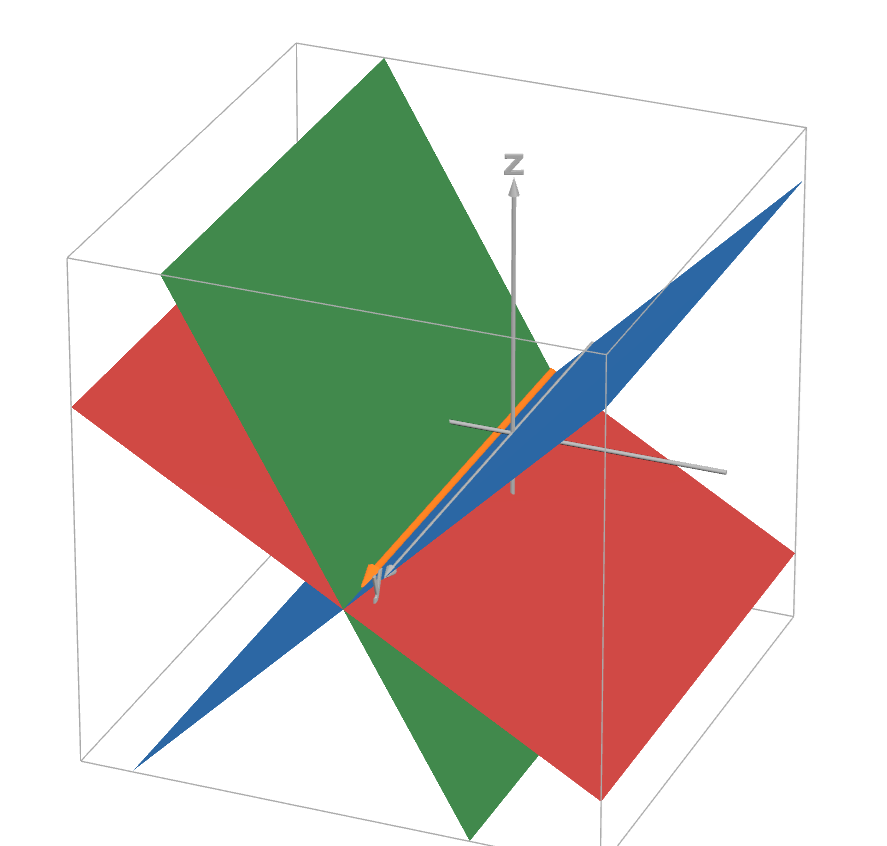
\includegraphics[scale=0.22]{Three Planes All In a Line.png}
        \caption*{Three planes, all in a line!}
    \end{figure}
\end{minipage}
\hfill
\begin{minipage}{0.48\textwidth}
    \begin{center}or be all the same plane!\end{center}
    \vspace{-1em}
    \begin{align*}
        3x + 2y - z &= 5 \\
        12x + 8y - 4z &= 20 \\
        x + \frac{2}{3}y - \frac{1}{3}z &= \frac{5}{3}
    \end{align*}
    \begin{figure}[H]
        \centering
        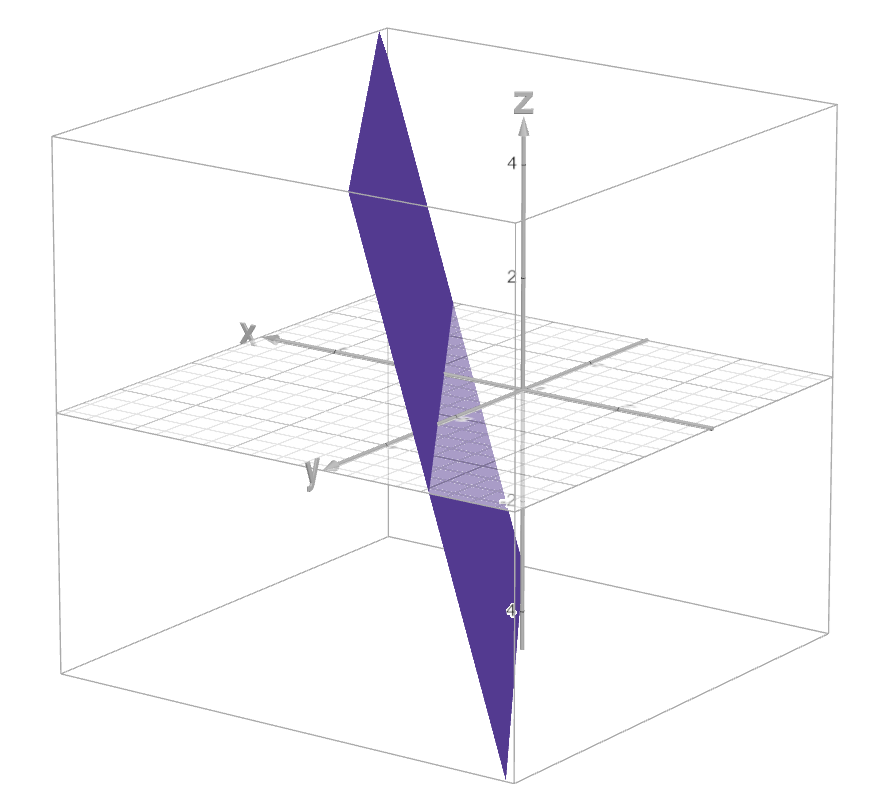
\includegraphics[scale=0.21]{All Just One Plane.png}
        \caption*{It's all the same plane.}
    \end{figure}
\end{minipage}

\newpage
So while you need $n$ equations for $n-1$D planes to have 1 solution, you could still have a solution that is of higher dimension. Less abstractly, 2D planes need 3 equations to have a signle solution, but even with 2 equations, we may have a 1D plane or a 2D plane as our solution.

When looking at the initial matrices,
\begin{align*}
    \begin{bmatrix}[ccc|c]
    1 & 0 & -\sqrt3 & 2 \\
    1 & 0 & 1 & 0 \\
    \sqrt3 & 0 & -1 & 2
    \end{bmatrix}
    &&
    \begin{bmatrix}[ccc|c]
        3 & 2 & -1 & 5 \\
        12 & 8 & -4 & 20 \\
        1 & \frac{2}{3} & \frac{1}{3} & \frac{5}{3}
    \end{bmatrix},
\end{align*}
it's relatively easy to tell the right matrix will have the whole plane as a solution. The left matrix being just a line? Less obvious. Let's row-reduce the left matrix:
\begin{align*}
    \begin{bmatrix}[ccc|c]
        1 & 0 & -\sqrt3 & 2 \\
        1 & 0 & 1 & 0 \\
        \sqrt3 & 0 & -1 & 2
    \end{bmatrix}
    \xto[R_2 \to R_2 - R_1][R_3 \to R_3 - \sqrt 3 R_1]&
    \begin{bmatrix}[ccc|c]
        1 & 0 & -\sqrt{3} & 2 \\
        0 & 0 & 1 + \sqrt3 & -2 \\
        0 & 0 & -1 + 3 = 2 & 2(1 - \sqrt3)
    \end{bmatrix}\\
    \xto[R_3 \to R_3/2]&
    \begin{bmatrix}[ccc|c]
        1 & 0 & -\sqrt{3} & 2 \\
        0 & 0 & 1 + \sqrt3 & -2 \\
        0 & 0 & 1 & 1 - \sqrt3
    \end{bmatrix}
\end{align*}
Almost at row-echelon form! Continuing to simplify:
\begin{align*}
    \begin{bmatrix}[ccc|c]
        1 & 0 & -\sqrt{3} & 2 \\
        0 & 0 & 1 + \sqrt3 & -2 \\
        0 & 0 & 1 & 1 - \sqrt3
    \end{bmatrix}
    \xto[R_2 \to R_2 - R_3]&
    \begin{bmatrix}[ccc|c]
        1 & 0 & -\sqrt3 & 2 \\
        0 & 0 & \sqrt3 & -3 + \sqrt3 \\
        0 & 0 & 1 & 1 - \sqrt3
    \end{bmatrix} \\
    \xto[R_2 \to R_2 - \sqrt3 R_3]&
    \begin{bmatrix}[ccc|c]
        1 & 0 & -\sqrt3 & 2 \\
        0 & 0 & 0 & 0 \\
        0 & 0 & 1 & 1 - \sqrt3
    \end{bmatrix} \\
    \xto[R_3 \lrto R_2]&
    \begin{bmatrix}[ccc|c]
        1 & 0 & -\sqrt{3} & 2 \\
        0 & 0 & 1 & 1 - \sqrt3 \\
        0 & 0 & 0 & 0
    \end{bmatrix}
\end{align*}
We got a row of all 0s. This means our system of equations is equivalent to a system of equations of 2 equations, which means that it's impossible for us to have a single point as a solution as we need 3 planes to get a point. And because the second column has no leading 1s, we know it's a free variable. So while you usually can't recognize a system of equations does not have a unique solution (aka a single point) from the original equations, row-echelon form reveals all by manipulating our equations until we can get rid of equations that do not add any new information.

In the second matrix from earlier, because rows 2 and row 3 are scalar multiples of row 1, we have
\[
    \begin{bmatrix}[ccc|c]
        3 & 2 & -1 & 5 \\
        12 & 8 & -4 & 20 \\
        1 & \frac{2}{3} & \frac{1}{3} & \frac{5}{3}
    \end{bmatrix}
    \longrightarrow
    \begin{bmatrix}[ccc|c]
        3 & 2 & -1 & 5 \\
        0 & 0 & 0 & 0 \\
        0 & 0 & 0 & 0
    \end{bmatrix}
\]
We see that columns 2 and 3 have no leading 1. Thus they are free variables, as we have $x = (5 - 2y + z)/3$. Think of free variables as independent variables. $x$ depends on $y$ and $z,$ so $y$ and $z$ are free to be any numbers we wish while $x$ will change accordingly. Because we have two 0 rows, we only have one equation, so our solution has to be just a full 2D plane.

How else could you get 3 equations yet a line as a solution? One way is equations being multiples of each other Another way is one equation is just the sum of the others:
\begin{align*}
    \begin{aligned}
    5x + 3y -2z = -1 \\
    -x + 2y + 9z = 8 \\
    4x + 5y + 7z = 7.
    \end{aligned}
    &&
    \begin{bmatrix}[ccc|c]
        5 & 3 & -2 & -1 \\
        -1 & 2 & 9 & 8 \\
        4 & 5 & 7 & 7
    \end{bmatrix}
\end{align*}
Here, row 3 is the sum of row 1 and row 2. When we row-reduce, you can see how the last row will become all 0s quickly, guaranteeing that some column won't have a \textit{pivot point} (another term for a leading 1) because we have 3 variables and 3 equations/rows so one pivot point would have had to have been in the final row. So once again, while there was cluses that the matrix would have a free variable in its initial form, row-echelon form makes it obvious.

Other matrices that do not have a unique solution will have equations that are sums and multiples of the other equations combined together, making the matrices lack of a unique solution even less obvious:
\begin{align*}
    \begin{aligned}
    5x + 3y -2z = -1 \\
    -x + 2y + 9z = 8 \\
    8x + 2y - 22z = -18
    \end{aligned}
    &&
    \begin{bmatrix}[ccc|c]
        5 & 3 & -2 & -1 \\
        -1 & 2 & 9 & 8 \\
        8 & 2 & -22 & -18
    \end{bmatrix}
\end{align*}
Here, row 3 is equal to $2R_1 - 2R_2.$ So again, there will be a 0 row at the end, yet it's not obvious at all at the start. Tricky, huh? So row-echelon form is what let's us see the truth by solving the system!

We'll explore this concept of a point solution not being reached despite having enough equations in the next unit. When equations do not have a unique solution despite there being enough equations to do so, the equations are called \textit{linearly independent}.

\subsubsection*{Overview}
\begin{itemize}
    \item Solutions represent intersections of planes. In $n$ dimensions with $n$ nonzero equations, our solution can be a $n-1$ dimesional plane at highest.
    \item You can't really tell what dimension a matrix's solution will be until after row-reducing.
    \item $n$ by $n$ matrices that do not have a point solution may be that way because one equation is equal to sum of multiples of other equations. This sum is called a \textit{linear combination}, as we'll get into next unit.
    \item The number of free variables is what decides the dimension of the solution. If there's 1 free variable, for example, we'll have a line solution, and that typically means that 1 out of our 3 equations is a sum of the other equations/planes and doesn't add anything new.
\end{itemize}

\newpage
\section*{How Free Variables Affects Our Solution}
At this point, you may see an observation regarding how the number of free variables affects whether we have a point as our solution. 0 free variables means a 0D plane as a solution. 1 free variable means a 1D plane as a solution. And 2 free variables mean a 2D plane as a solution.

Let $A$ be a matrix for a system of equations. Let $\nullity A$ represent the number of free variables. Let $\dim(A)$ represent the number of variables, aka the number of columns in the matrix. This represents the dimension we're in, so 3 variables means 3 dimensions. Let $\rank(A)$ be the number of non-free variables. Then
\[\dim(A) = \rank(A) + \nullity(A)\]
This is called the rank-nullity theorem, and it is argubly the most important theorem of linear algebra. Yet at its core, it is obvious. The number of independent variables and the number of dependent variables equals the number of variables, duh. But geometrically, it's implications are intense, as we'll see in future units.

$\rank(A)$ can be thought of how close the matrix is to getting one solution. If $\nullity(A) = 0$, then $\rank(A) = \dim(A),$ the max value, and we call it full rank. Let's simplify things by letting $\dim(A) = 3.$ If we have no free variables, then we have full rank, and we have a unique solution, the smallest (and often considered best, hence the name ``rank'') result in 3D space.  But if we have 1 free variable, then our solution is a 1D plane, and our rank drops to 2. Then 2 free variables means our rank is 1, and our solution is a 2D plane. Finally, if all our variables are free, it actually means our solution is all of 3D space, and our rank is 0. This happens with equations like $0x + 0y + 0z = 0.$

Inversely, $\nullity(A)$ increases with each additional free variable, so it increases as we get farther away from our best result of a unique solution. At full nullity, the rank is 0, and all the variables are free. The solution is all of 3D space, as dicussed in the prevous paragraph. At 0 nullity, the rank is full, and no variables are free as we have a unique solution in 3D space. Why we call it nullity we'll be revealed in due time. For now, you can remember it with the silly phrase that more free variables means less rank and more ``badness'', more nullness.

\subsubsection*{Overview}
\begin{itemize}
    \item $\dim(A)$ is the number of columns, aka the number of variables in the system of equations.
    \item $\rank(A)$ is how close we are to unique solution. It's the number of non-free variables. Full rank happens when the rank equals the dimension, and we have a unique solution.
    \item $\nullity(A)$ is the number of free variables. It's the dimension of the solution space.
    \item $\dim(A) = \rank(A) + \nullity(A).$
\end{itemize}

\newpage
\section*{Tips for Guass-Jordan Elimination}
Go read \textbf{Solving a System of Equations} first, as it demonstrates when swapping rows will be beneficial.

While generally we want to avoid creating fractions for as long as possible, sometimes they are useful. Consider the following system:
\[
\begin{bmatrix}
    2 & 8 & -6 & 5 \\
    7 & 2 & 1 & 4 \\
    -4 & 3 & 2 & -1
\end{bmatrix}
\]
Which row is closet to 1? Well, 2 is, but it's still not 1. But hang on: all of row 1 are multiples of 2 except for the 5. Perhaps creating a fraction here is still worth it:
\[
    \begin{bmatrix}
        2 & 8 & -6 & 5 \\
        7 & 2 & 1 & 4 \\
        -4 & 3 & 2 & -1
    \end{bmatrix}
    \xto[R_1 \to R_1/2]
    \begin{bmatrix}
        1 & 4 & -3 & 5/2 \\
        7 & 2 & 1 & 4 \\
        -4 & 3 & 2 & -1.
    \end{bmatrix}
\]
    Because we only have a fraction in one column, the math isn't too bad, so it was worth dividing here.

    Other times, you'll be able to tell how you could create a 1 by adding rows together:
    \[
        \begin{bmatrix}
            2 & 8 & -5 & 5 \\
            -3 & 4 & -1 & 3 \\
            -4 & 3 & 2 & -1
        \end{bmatrix}
    \]
    Here, $2 - 3 = -1,$ so what we should do is $R_1 \to -(R_1 + R_2) = -R_1 - R_2$:
    \[
        \begin{bmatrix}
            1 & -12  & 6 & -8 \\
            -3 & 4 & -1 & 3 \\
            -4 & 3 & 2 & -1
        \end{bmatrix}
    \]
    From here, we could ellimiate row 3 by adding 3 of row 1 and we coul eliminate row 2 by adding 4 of row 1. Let's add 4 of row 1 to create a 0 in row 3:
    \[
        \begin{bmatrix}
            1 & -12  & 6 & -8 \\
            -3 & 4 & -1 & 3 \\
            -4 & 3 & 2 & -1
        \end{bmatrix}
        \xto[R_3 \to R_3 + 4R_1]
        \begin{bmatrix}
            1 & -12  & 6 & -8 \\
            -3 & 4 & -1 & 3 \\
            0 & -45 & 26 & -33 
        \end{bmatrix}
    \]
    One way you can also save time is instead of creating the 1 in the top row first, if you see an easy way to create a 0 later in the column, you could do that first before creating the 1:
    \begin{align*}
        \begin{bmatrix}
            2 & 8 & -5 & 5 \\
            -3 & 4 & -1 & 3 \\
            -4 & 3 & 2 & -1
        \end{bmatrix}
        \xto[R_3 \to R_3 + 2R_3]&
        \begin{bmatrix}
            2 & 8 & -5 & 5 \\
            -3 & 4 & -1 & 3 \\
            0 & 19 & 8 & 9
        \end{bmatrix} \\
        \xto[R_1 \to -R_1 - R_2]
        \begin{bmatrix}
            1 & -12 & 6 & -8 \\
            -3 & 4 & -1 & 3 \\
            0 & 19 & 8 & 9
        \end{bmatrix}
    \end{align*}
    This way, we didn't have to add 4 of a row and instead added 2 of a row to create a 0 in row 3. This meant easier multiplication in our heads and the numbers in row 3 are smaller and easier to work with.

    \subsubsection*{Overview}
    \begin{itemize}
        \item Swapping rows can bring the 1s to the right spot.
        \item Consider dividing if most entries in a row have a common factor
        \item Add rows that create 1 or -1. Consider also creating 0s in the column before creating the 1s if you're able to as it might make the math easier.
    \end{itemize}

\end{document}